\section{Malliavin Calculus}\label{apx:malliavin_calculus}

We provide a brief introduction to these concepts and tools in this section. However, for a more in-depth understanding of this field, we recommend referring to Nualart~\cite{Nualart2006TheTopics}. Malliavin calculus deals with the study of the differentiability properties of random variables, particularly those defined on a Wiener space. The calculus uses a differentiation operator called the Malliavin derivative, which is defined with respect to the underlying Brownian motion. The Malliavin derivative operator is a powerful tool that enables us to compute derivatives of stochastic integrals. This is especially useful in finance, where stochastic integrals are commonly used to model complex financial products. By applying the Malliavin derivative operator to stochastic integrals, we can derive formulas for the sensitivities of these products to their underlying parameters, such as interest rates, volatilities, and maturities. Let now $\SSb$ be the set of random variables of the form
\[
F=f\left(W\left(h_1\right), \ldots, W\left(h_n\right)\right)
\]
with $(h_1, \ldots, h_n) \in L^2([0, T]), W\left(h_i\right)$ denoting the Wiener integral of the function $h_i$, for $i\in\{1, \dots, n\}$, and $f \in \Cc_b^{\infty}\left(\RR^n\right)$. The Malliavin derivative of $F$ is defined as the stochastic process in $L^2(\Omega \times[0, T])$ given by
\[
\Dr_s F=\sum_{j=1}^n \frac{\partial f}{\partial x_j}\big(W\left(h_1\right), \ldots, W\left(h_n\right)\big)(s) h_j(s)
\]
We can also define the iterated Malliavin derivative operator as
\[
\Dr_{s_1, \dots, s_m}^m F = \Dr_{s_1} \dots \Dr_{s_m} F, \quad s_1, \dots, s_m \in[0, T]\,.
\]
These operators are closable in~$L^p(\Omega)$ for any~$p \geq 1$ and we denote by $\DD^{n, p}$ the closure of $\SSb$ with respect to the norm
\[
\|F\|_{n, p}=\left(\EE\left[|F|^p\right]+\sum_{i=1}^n \EE\left[\left\|\Dr^i F\right\|_{L^2\left([0, T]^i\right)}^p\right]\right)^{\frac{1}{p}}\,.
\]
The above definition can be extended to the case of random variables with values in $L^2([0, T])$. Let us also consider the class~$\SSb_{L^2([0, T])}$ of $L^2([0, T])$-valued random variables of the form
\[
\sum_{i=1}^n F_i h_i\,
\]
where $F_i \in \SSb$, and $h_i \in L^2([0, T])$ for $i\in\{1,\dots n\}$. Then, we denote by~${\LL^{n, p}= \DD_W^{n, p}\left(L^2([0, T])\right)}$ the completion of $\SSb_{L^2([0, T])}$ by the norm
\[
\|F\|_{n, p, L^2([0, T])}=\left(\EE\left[|F|_{L^2([0, T])}^p\right] + \sum_{i=1}^n \EE\left[\left\|D^i F\right\|_{L^2\left([0, T]^{i+1}\right)}^p\right]\right)^{\frac{1}{p}}\,.
\]
Finally, the following result gives us an explicit martingale representation for random variables in $\DD_W^{1,2}$. For the proof in one-dimensional case see e.g.~\cite[Proposition 1.3.14]{Nualart2006TheTopics}.
\begin{theorem}[Clark-Ocone formula]\label{thm:ClarkOcone}
Let a random variable $F \in \DD_W^{1,2}$, then the following decomposition holds 
\[
F = \EE[F] + \int_0^T \EE_s\left[\Dr_s F\right] \D W_s\,.
\]
\end{theorem}

\section{Empirical analysis of the VIX distribution}\label{apx:VIX_smile_rBergomi}

This appendix section focuses on the empirical analysis of the~VIX distribution, challenging the assumption commonly employed in mathematical finance models that the~VIX follows a Log-Normal distribution. By conducting a statistical examination of the VIX time series, we aim to provide evidence contrary to this assumption. 

For instance, consider the volatility process of the rough Bergomi model, represented by the equation:
\[
V_t = \xi_0(t) \Ee^\lozenge\left(\eta_H B_t^{H}\right), \qquad V_0>0\,,
\]
where~$B_t^{H}$ denotes the fractional Brownian motion with Hurst parameter $H\in(0,1)$. Since $B_t^{H}$ is a Gaussian process, the volatility exhibits Log-Normal dynamics, resulting in the VIX under the rough Bergomi model being distributed as a sum of Log-Normal variables, which is, by Fenton-Wilkinson approximation~\cite{Fenton1960TheSystems}, again close to Log-Normal. Nevertheless, our empirical analysis suggests that the VIX distribution does not align closely with a Log-Normal distribution, thereby challenging the prevailing assumption.

Examining the distribution of log-returns based on daily CBOE data spanning from Jan~3,~2005, to October~28,~2022, in Figure~\ref{fig:VIX_dist}, it is at first apparent that the majority of its characteristics can be approximated by a normal distribution. However, a more careful look reveals the presence of residual skewness and kurtosis that cannot be fully accounted for within the confines of a standard normal model.

\begin{figure}[htbp]
    \centering
    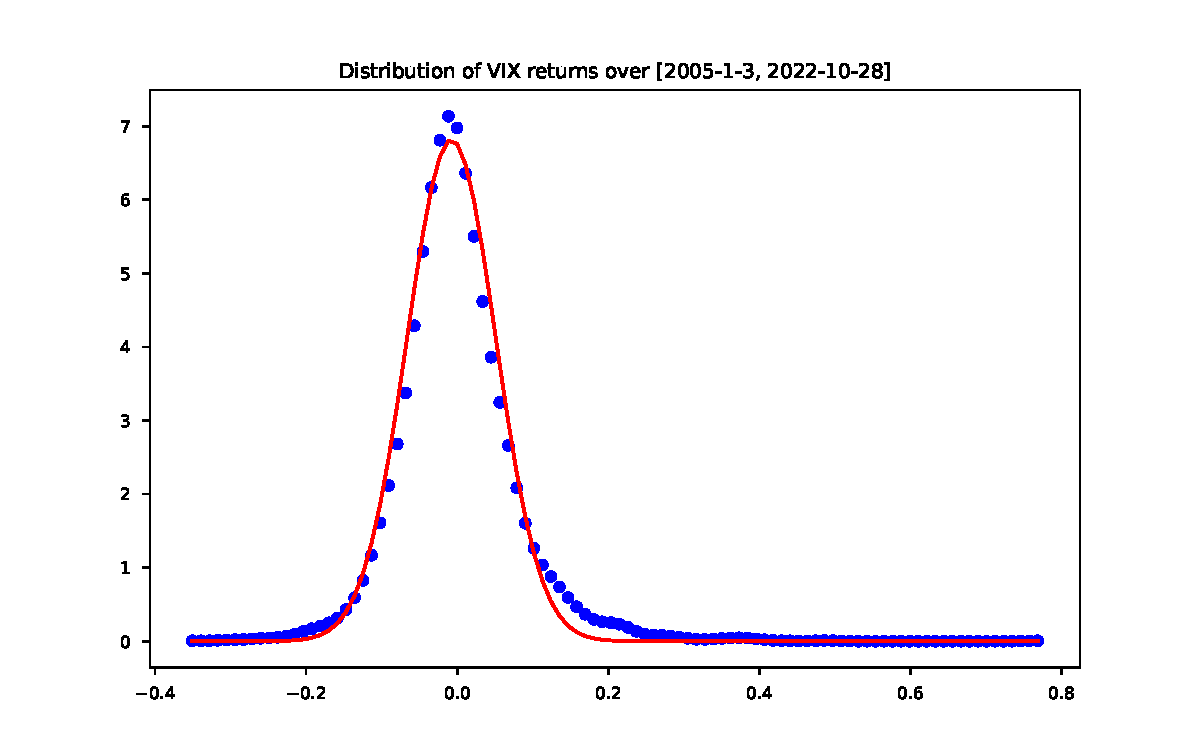
\includegraphics[width=\textwidth]{content/reschap4/Figures/VIX_dist_2005-1-3-2022-10-28.pdf}
    \centering
    \begin{subfigure}[b]{\textwidth}
        \centering
        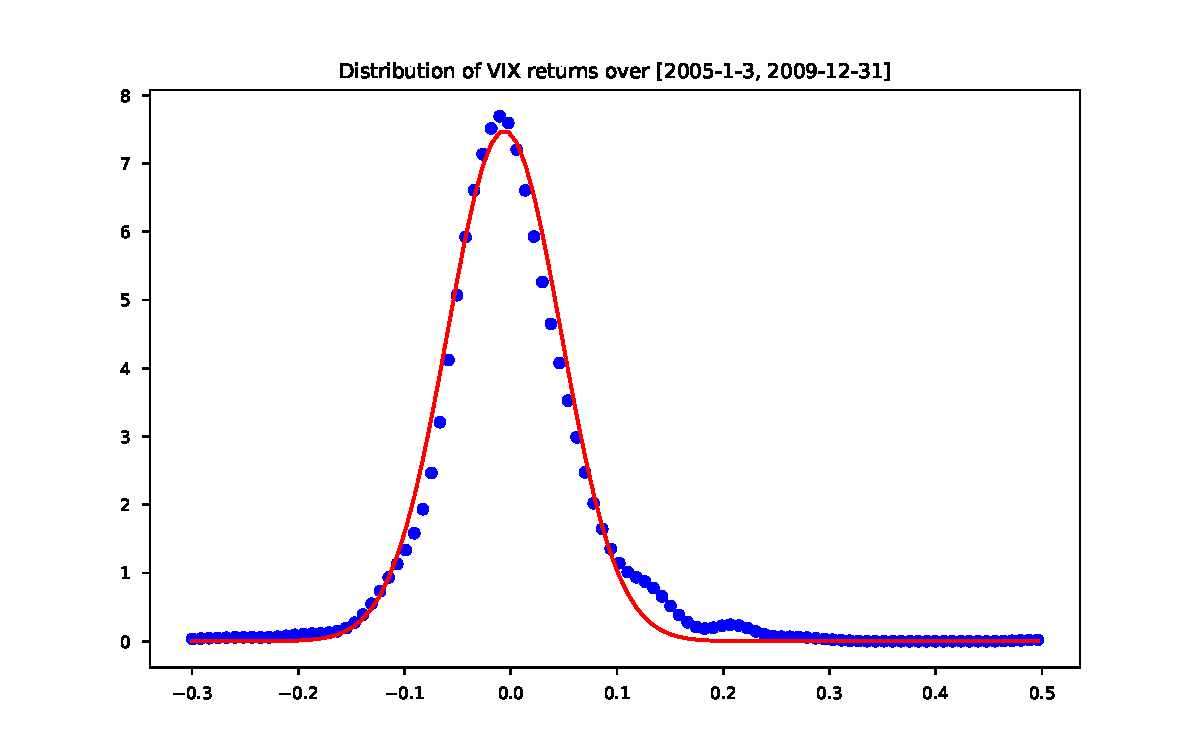
\includegraphics[width=0.45\textwidth]{content/reschap4/Figures/VIX_dist_2005-1-3-2009-12-31.pdf}
        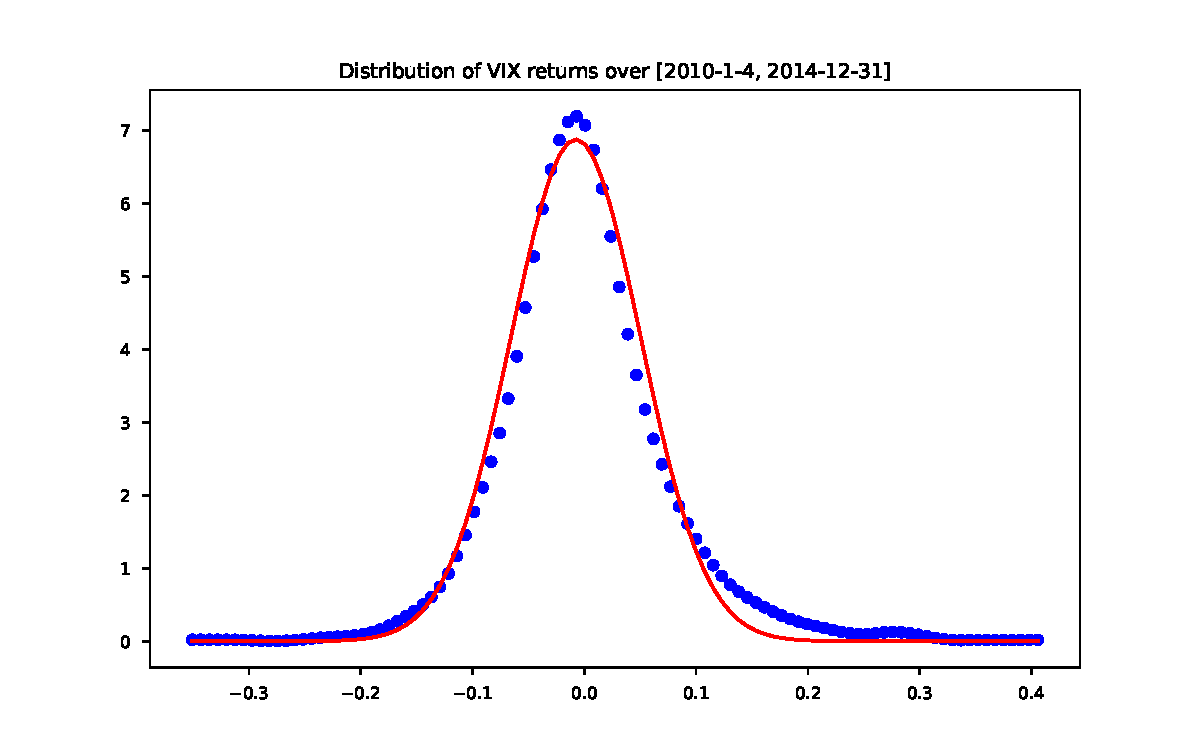
\includegraphics[width=0.45\textwidth]{content/reschap4/Figures/VIX_dist_2010-1-4-2014-12-31.pdf}
        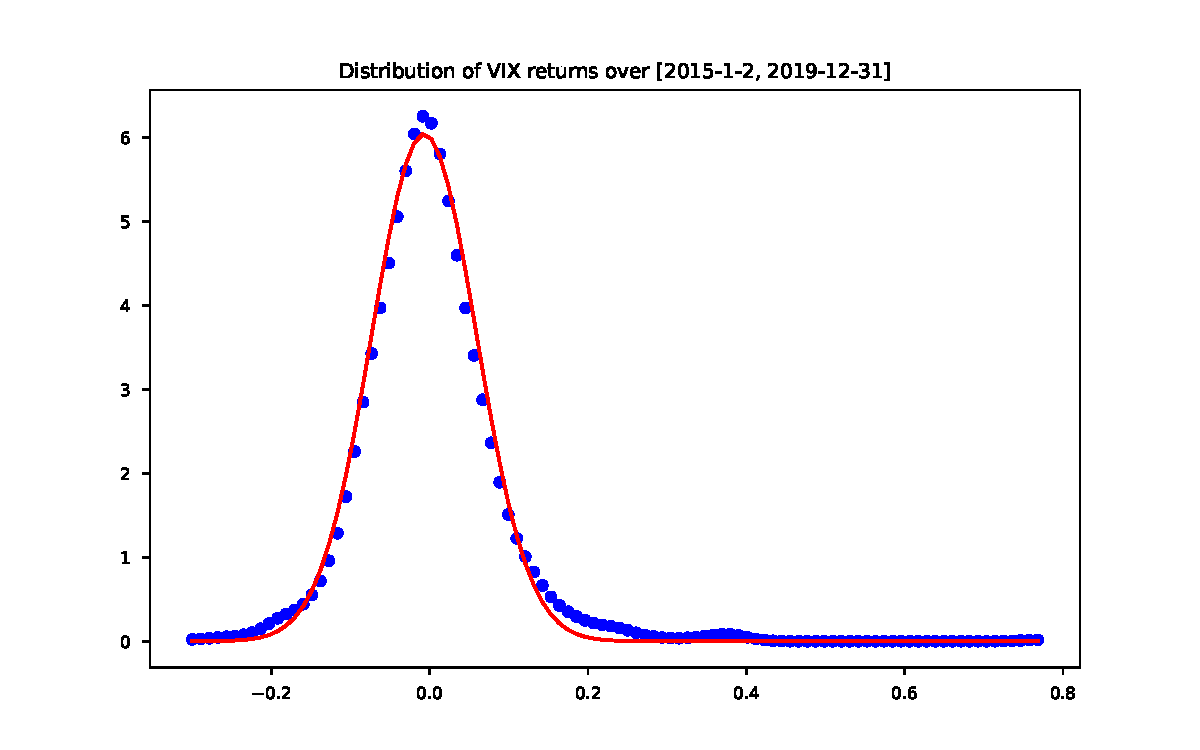
\includegraphics[width=0.45\textwidth]{content/reschap4/Figures/VIX_dist_2015-1-2-2019-12-31.pdf}
        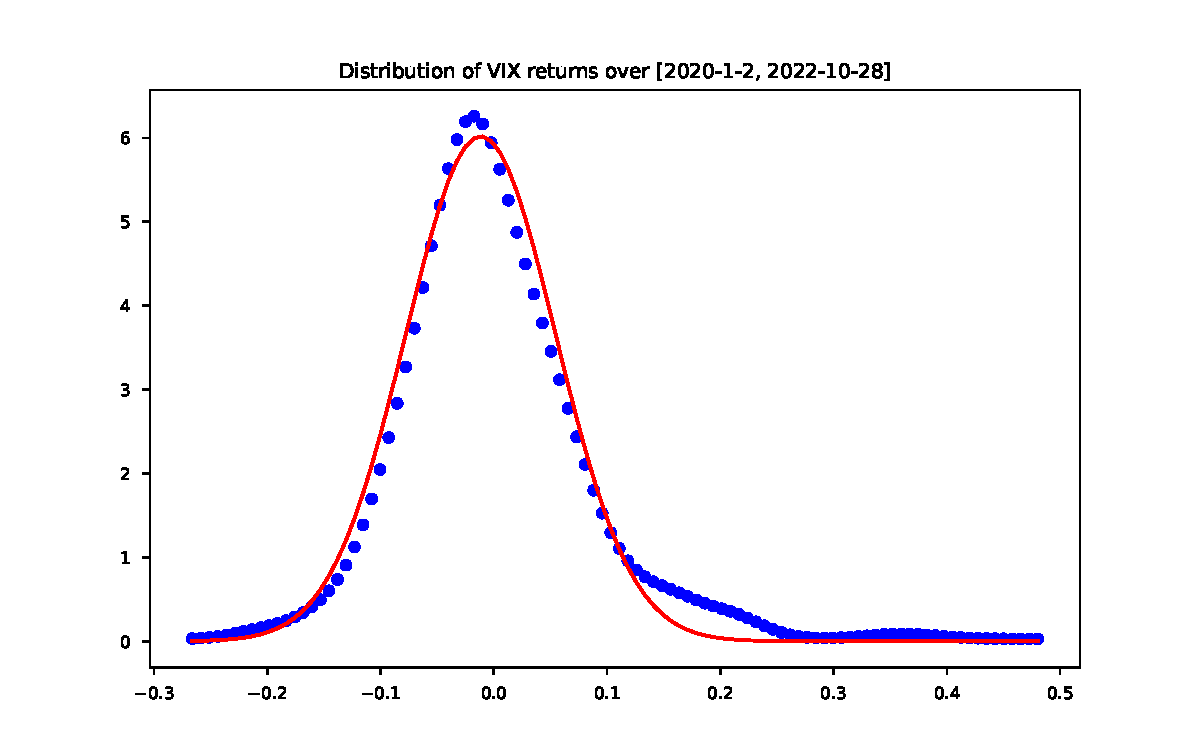
\includegraphics[width=0.45\textwidth]{content/reschap4/Figures/VIX_dist_2020-1-2-2022-10-28.pdf}
    \end{subfigure}
    \caption{\textit{Top}: the fit of Gaussian distribution to empirical log-returns of VIX over the period 2005-01-03 to 2022-10-28. \textit{Bottom}: the fit over periods 2005-2010, 2010-2015, 2015-2020.}
    \label{fig:VIX_dist}
\end{figure}

Next, through a comparative analysis of VIX log-returns using quantile-quantile~(QQ) plots in Figure~\ref{fig:QQplots}, we examine the suitability of various probability distributions, including the normal, Student's~t, and Laplace distributions over different periods. The results reveal that while the normal distribution fails to capture the tail behaviour of VIX returns, both the Student's t and Laplace distributions exhibit improved fit in the tails. However, a notable limitation is observed in the inability of these distributions to capture the asymmetry present in the VIX returns fully, although the severity of miss-fit differed throughout different periods.

\begin{figure}[htbp]
    \centering
    \begin{subfigure}[b]{0.32\textwidth}
        \centering
        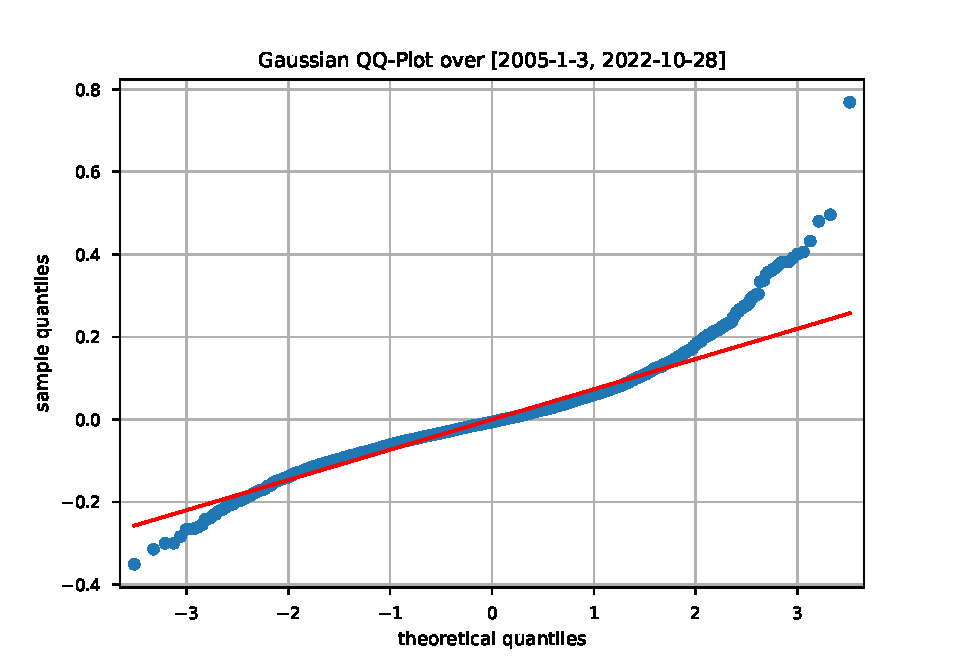
\includegraphics[width=\textwidth]{content/reschap4/Figures/gauss_QQ_2005-1-3-2022-10-28.pdf}
        \caption{Gaussian}
        % \label{fig:image1}
    \end{subfigure}
    \hfill
    \begin{subfigure}[b]{0.32\textwidth}
        \centering
        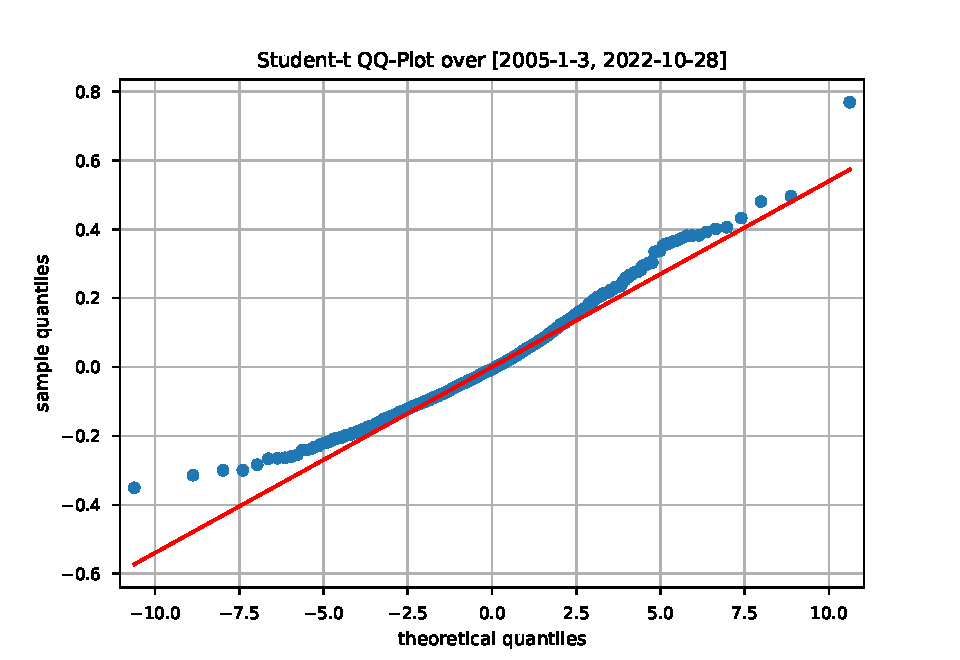
\includegraphics[width=\textwidth]{content/reschap4/Figures/student_QQ_2005-1-3-2022-10-28.pdf}
        \caption{Student's t}
        % \label{fig:image2}
    \end{subfigure}
    \hfill
    \begin{subfigure}[b]{0.32\textwidth}
        \centering
        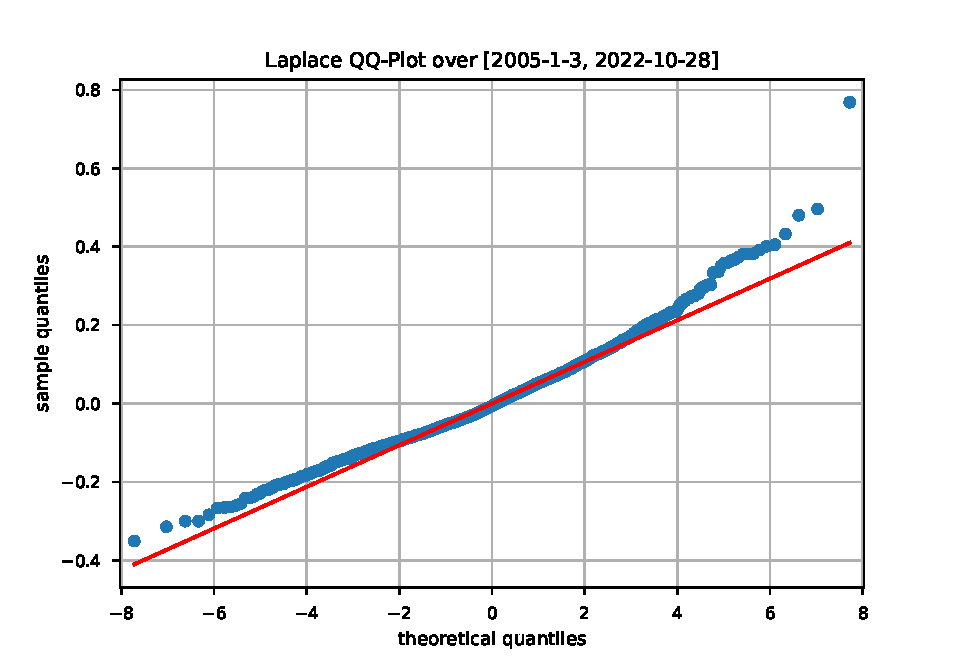
\includegraphics[width=\textwidth]{content/reschap4/Figures/laplace_QQ_2005-1-3-2022-10-28.pdf}
        \caption{Laplace}
        % \label{fig:image3}
    \end{subfigure}

    \centering
    \begin{subfigure}[b]{0.32\textwidth}
        \centering
        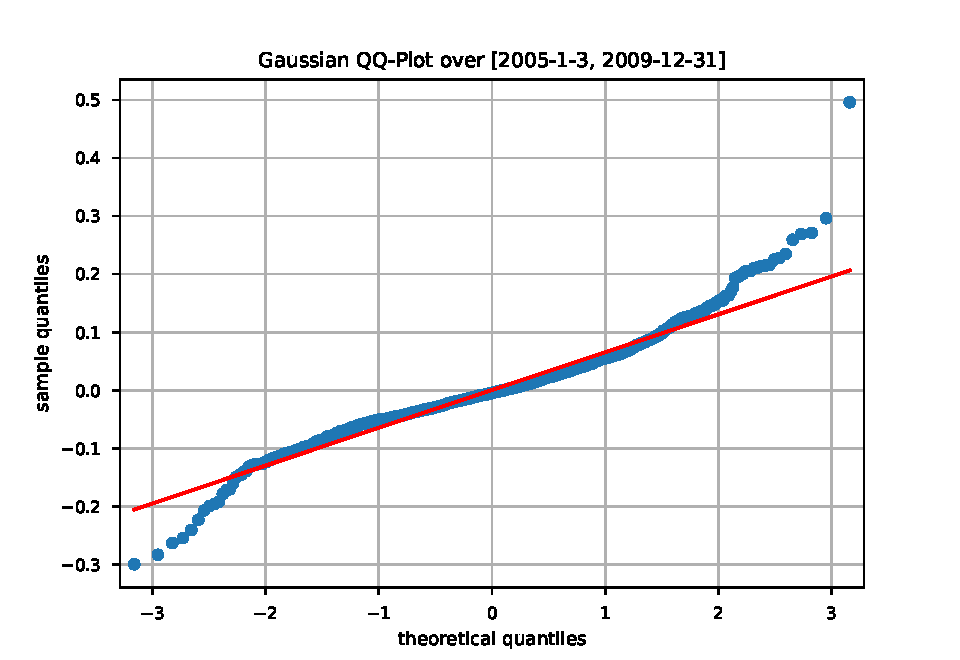
\includegraphics[width=\textwidth]{content/reschap4/Figures/gauss_QQ_2005-1-3-2009-12-31.pdf}
        \caption{Gaussian}
    \end{subfigure}
    \hfill
    \begin{subfigure}[b]{0.32\textwidth}
        \centering
        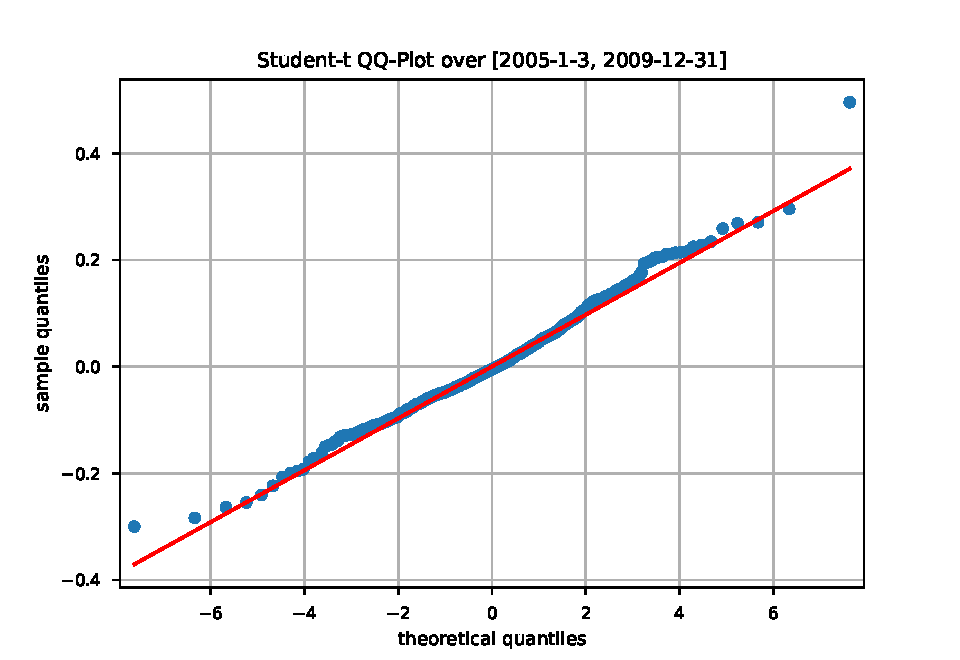
\includegraphics[width=\textwidth]{content/reschap4/Figures/student_QQ_2005-1-3-2009-12-31.pdf}
        \caption{Student's t}
    \end{subfigure}
    \hfill
    \begin{subfigure}[b]{0.32\textwidth}
        \centering
        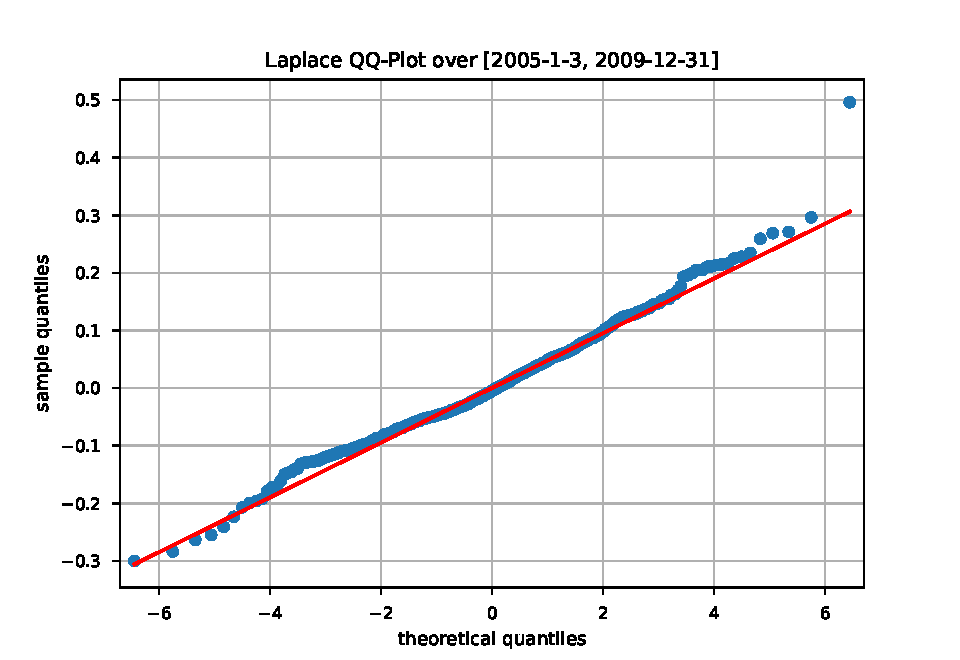
\includegraphics[width=\textwidth]{content/reschap4/Figures/laplace_QQ_2005-1-3-2009-12-31.pdf}
        \caption{Laplace}
    \end{subfigure}

    \centering
    \begin{subfigure}[b]{0.32\textwidth}
        \centering
        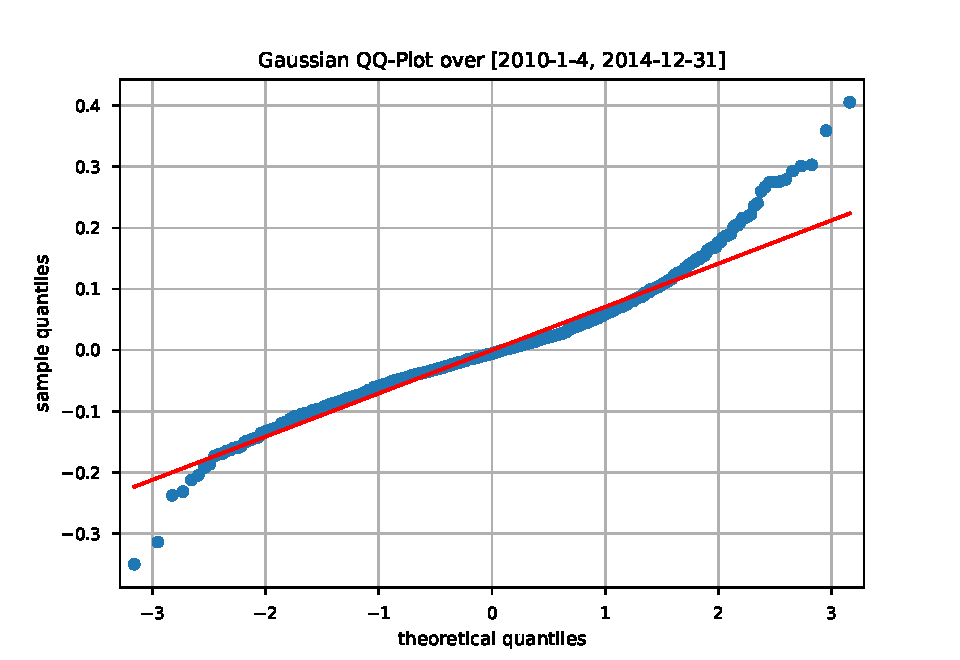
\includegraphics[width=\textwidth]{content/reschap4/Figures/gauss_QQ_2010-1-4-2014-12-31.pdf}
        \caption{Gaussian}
    \end{subfigure}
    \hfill
    \begin{subfigure}[b]{0.32\textwidth}
        \centering
        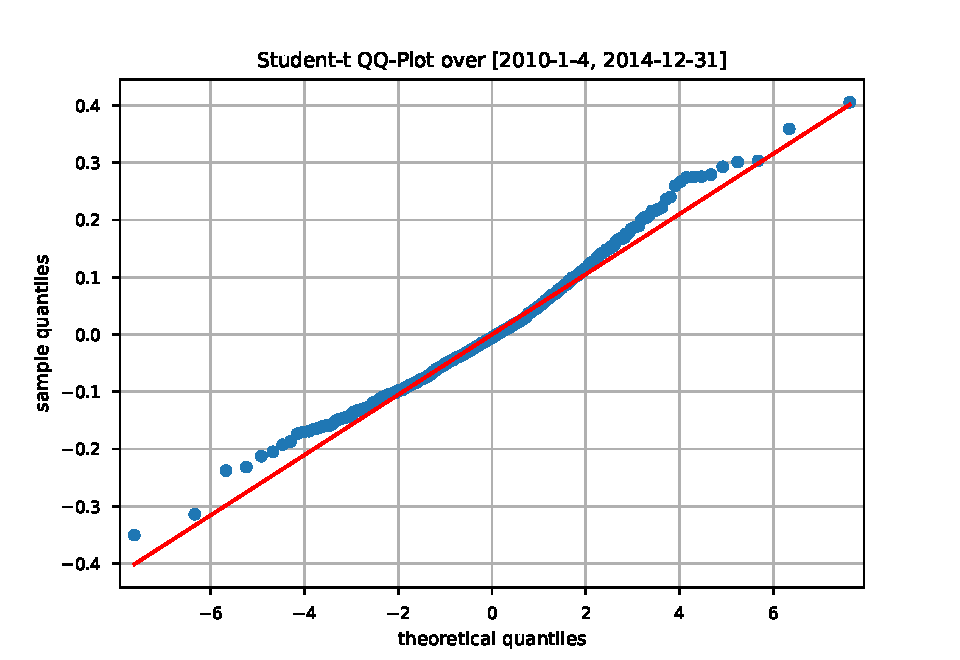
\includegraphics[width=\textwidth]{content/reschap4/Figures/student_QQ_2010-1-4-2014-12-31.pdf}
        \caption{Student's t}
    \end{subfigure}
    \hfill
    \begin{subfigure}[b]{0.32\textwidth}
        \centering
        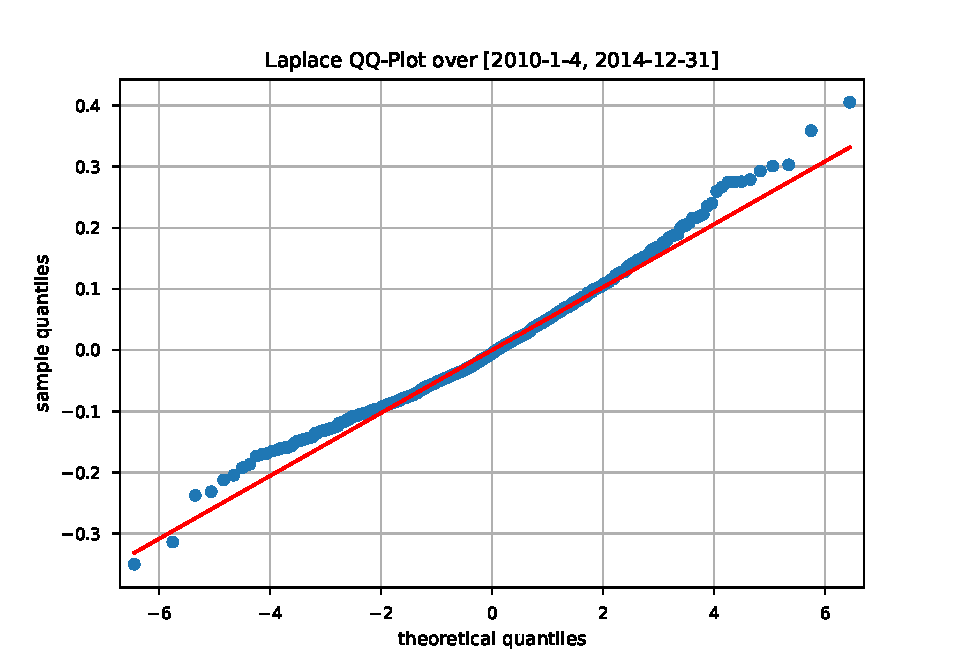
\includegraphics[width=\textwidth]{content/reschap4/Figures/laplace_QQ_2010-1-4-2014-12-31.pdf}
        \caption{Laplace}
    \end{subfigure}

    \centering
    \begin{subfigure}[b]{0.32\textwidth}
        \centering
        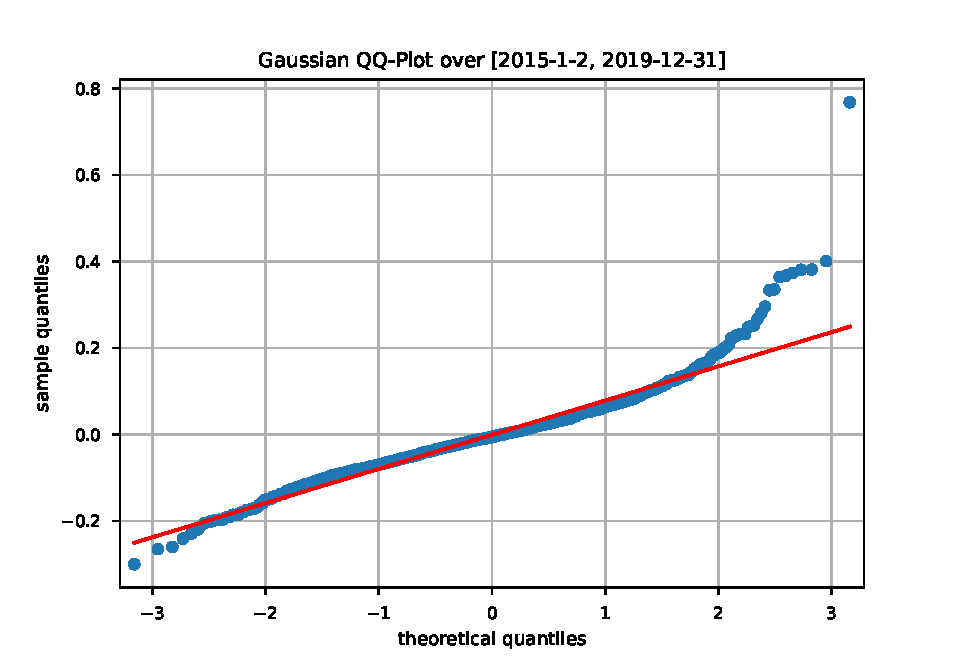
\includegraphics[width=\textwidth]{content/reschap4/Figures/gauss_QQ_2015-1-2-2019-12-31.pdf}
        \caption{Gaussian}
    \end{subfigure}
    \hfill
    \begin{subfigure}[b]{0.32\textwidth}
        \centering
        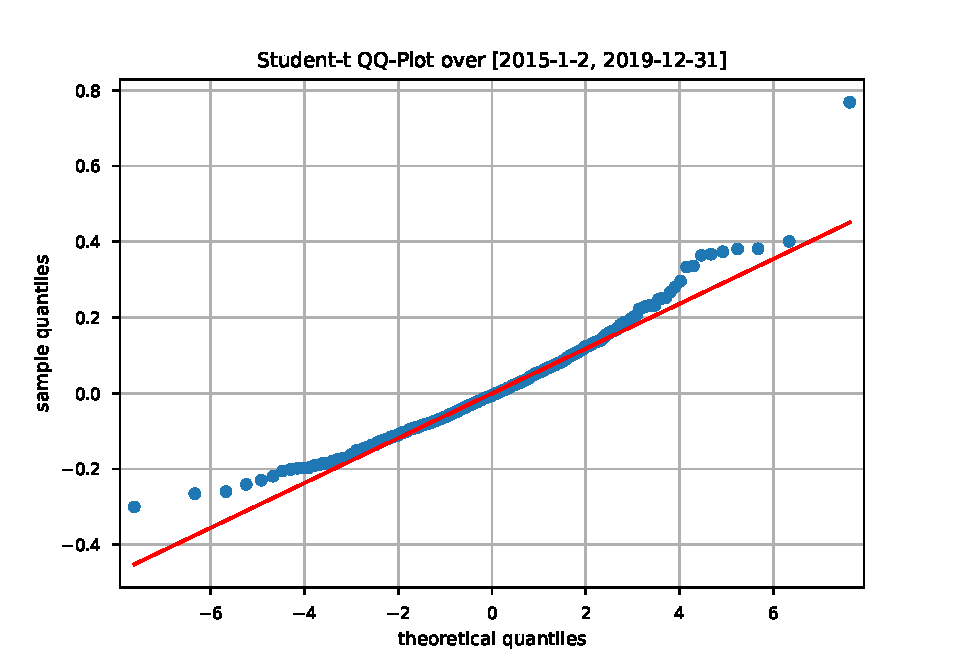
\includegraphics[width=\textwidth]{content/reschap4/Figures/student_QQ_2015-1-2-2019-12-31.pdf}
        \caption{Student's t}
    \end{subfigure}
    \hfill
    \begin{subfigure}[b]{0.32\textwidth}
        \centering
        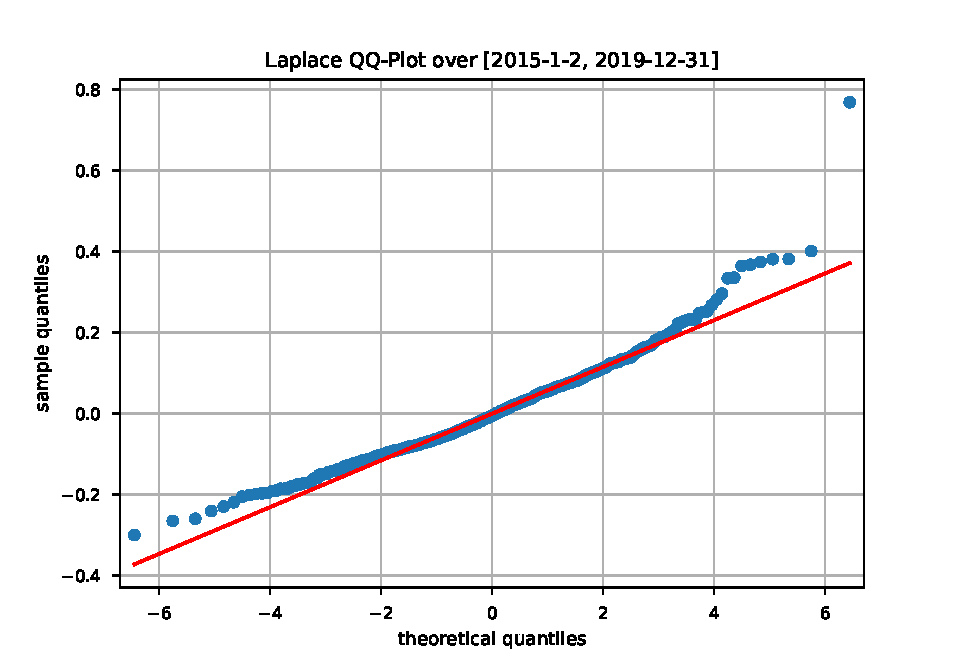
\includegraphics[width=\textwidth]{content/reschap4/Figures/laplace_QQ_2015-1-2-2019-12-31.pdf}
        \caption{Laplace}
    \end{subfigure}

    \centering
    \begin{subfigure}[b]{0.32\textwidth}
        \centering
        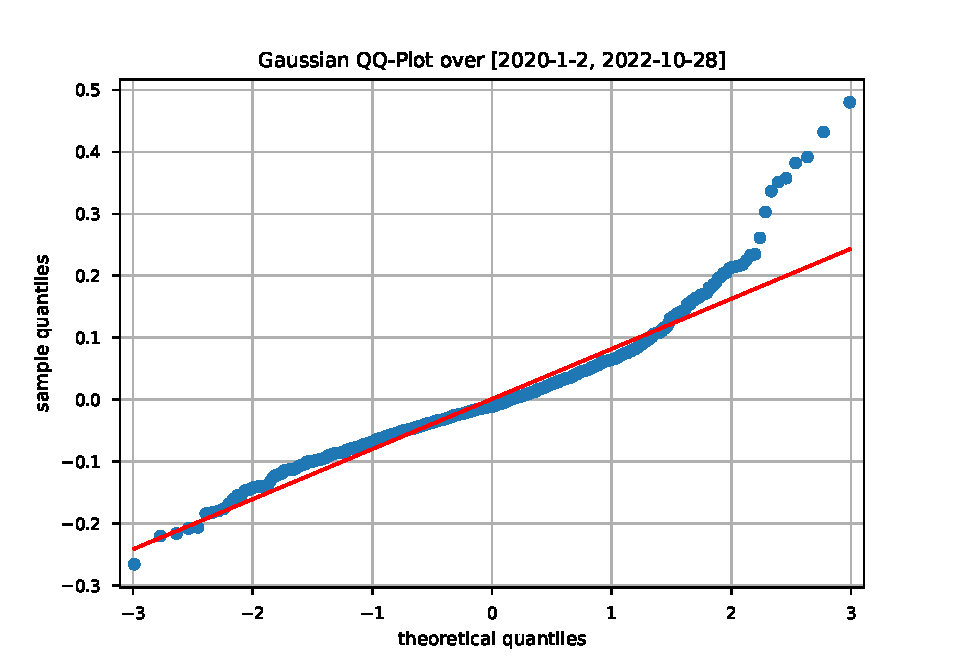
\includegraphics[width=\textwidth]{content/reschap4/Figures/gauss_QQ_2020-1-2-2022-10-28.pdf}
        \caption{Gaussian}
    \end{subfigure}
    \hfill
    \begin{subfigure}[b]{0.32\textwidth}
        \centering
        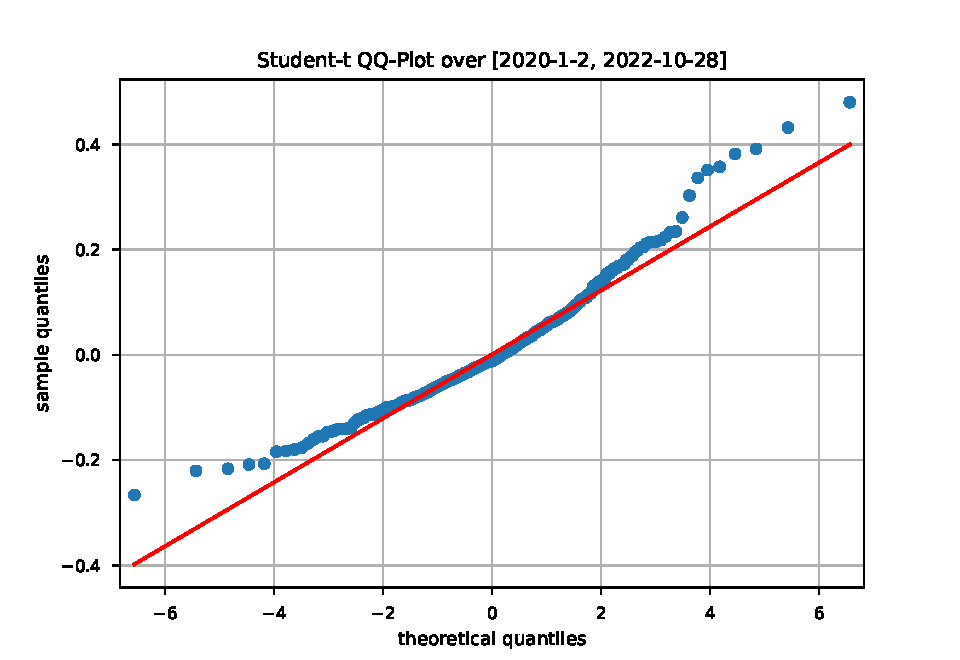
\includegraphics[width=\textwidth]{content/reschap4/Figures/student_QQ_2020-1-2-2022-10-28.pdf}
        \caption{Student's t}
    \end{subfigure}
    \hfill
    \begin{subfigure}[b]{0.32\textwidth}
        \centering
        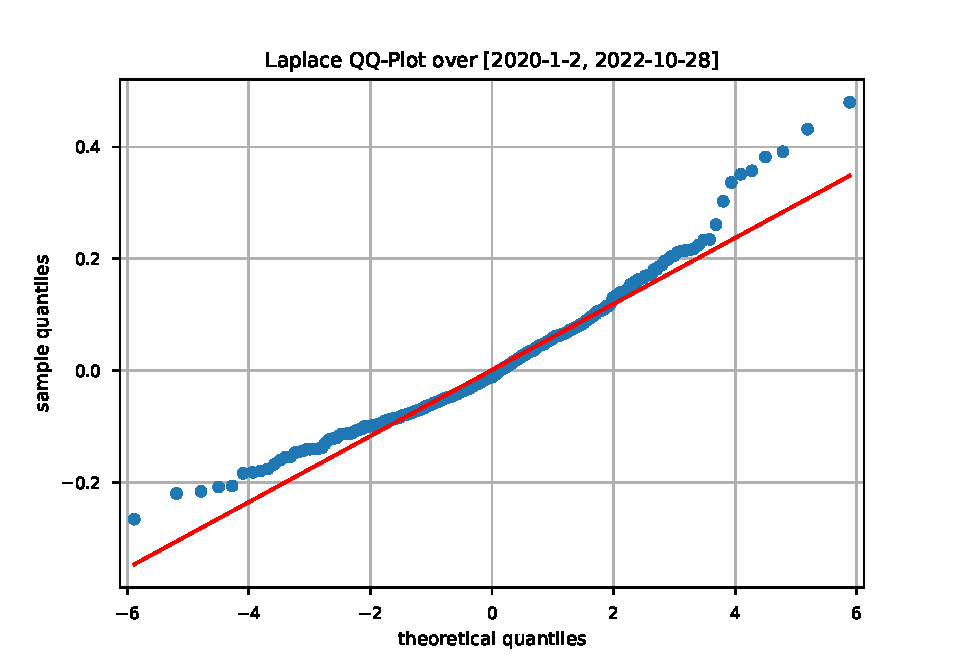
\includegraphics[width=\textwidth]{content/reschap4/Figures/laplace_QQ_2020-1-2-2022-10-28.pdf}
        \caption{Laplace}
    \end{subfigure}
    \caption{Comparing the tails of empirical VIX log-returns to the corresponding theoretical distributions using QQ plots over the following periods: (a)-(c)~{2005-01-03} to {2022-10-28}; (d)-(f)~{2005-01-03} to {2009-12-31}, (g)-(i)~{2010-01-04} to {2014-12-31}; (j)-(l)~{2015-01-02} to {2019-12-31}; (m)-(o)~{2020-01-02} to {2022-10-28}.}\label{fig:QQplots}
\end{figure}

Subsequently, we conduct several statistical tests to assess the normality of the returns over the same periods. Table~\ref{tab:normality_test} summarizes the results of the test for normality conducted on VIX log-returns. For the entire dataset, the skewness value is 1.048, accompanied by an extremely low {$p$\nobreakdash-value} from the test~\cite{DAgostino1990ANormality}, thus rejecting the null that the skewness of the population from which the sample was drawn is normal. Similarly, the (excess)~kurtosis value is 6.104, with a significantly low {$p$\nobreakdash-value} coming from the kurtosis test~\cite{Anscombe1983DistributionSamples}, thus again rejecting the null. These findings indicate substantial deviation from normality, as evidenced by the extremely low {$p$\nobreakdash-values}. Moreover, the norm test statistic based on~\cite{DAgostino1971AnSamples, DAgostino1973Testssqrtb_1} is zero up to machine precision, further supporting the rejection of the normality assumption for the VIX log-returns.

\begin{table}[]
\centerline{
\begin{tabular}{@{}llllll@{}}
\toprule
\textbf{Period}    & \textbf{Skewness} & \textbf{Skewness $p$-value} & \textbf{Kurtosis} & \textbf{Kurtosis $p$-value} & \textbf{Norm test} \\ \midrule
{2005-2022} & 1.05              & 2.24e-126                 & 6.10              & 6.68e-128                 & 1.36e-250          \\
{2005-2010} & 0.64              & 1.27e-17                  & 4.57              & 2.19e-31                  & 4.42e-46           \\
{2010-2015} & 0.70              & 3.32e-20                  & 3.37              & 1.49e-24                  & 7.47e-42           \\
{2015-2020} & 1.34              & 1.12e-51                  & 8.59              & 7.31e-48                  & 2.84e-96           \\
{2020-2022} & 1.28              & 8.08e-29                  & 4.62              & 1.93e-19                  & 2.51e-45 \\ \bottomrule
\end{tabular}
}
\caption{The table presents the outcomes of normality tests conducted on VIX log returns over different periods. The tests evaluate the skewness~\cite{DAgostino1990ANormality} and kurtosis~\cite{Anscombe1983DistributionSamples} of the underlying population compared to a normal distribution, as well as the overall adherence of the sample to a normal distribution~\cite{DAgostino1971AnSamples, DAgostino1973Testssqrtb_1}.
}\label{tab:normality_test}
\end{table}
Finally, we assessed the VIX returns' stationarity and employed the Augmented Dickey-Fuller test. We only report findings over the entire dataset, but the test results are persistent over different periods. The test yielded an Augmented Dickey-Fuller statistic of -24.01, accompanied by a $p$-value of zero. These results provide strong evidence against the null hypothesis of a unit root, indicating the presence of stationarity in the VIX returns. Furthermore, the critical values at the 1\% level (-3.432), 5\% level (-2.862), and 10\% level (-2.567) support the rejection of non-stationarity, reinforcing the robustness of the stationarity in the VIX returns.

We believe these findings underscore the importance of considering alternative distributional assumptions or more intricate models to comprehensively capture the unique characteristics of VIX returns, including both tail behaviour and asymmetry.


\section{Techical Proofs}\label{apx:technical_proofs}
\begin{lemma}\label{lem:sigma_prod}
Let $X, Y$ be two random variables on $(\Omega, \Ff)$ such that $X, Y \neq 0$ a.s.. Then, it holds for the generated sigma-algebra of the product that
$$
\sigma(X\cdot Y) \subseteq \sigma(X)\lor\sigma(Y)\,.
$$
\end{lemma}
\begin{proof}
Let $f(x, y)=x\cdot y$ and $\Bb\subseteq \Ff$ any Borel-measurable set. Then, since any continuous function is Borel measurable, $f^{-1}(\Bb)$ is a Borel set
% $$
% \{X Y \in B\}=\left\{(X, Y) \in f^{-1}(B)\right\}
% $$
\[
\{\omega:(X\cdot Y)(\omega) \in \Bb\}=\{\omega: f(X(\omega), Y(\omega)) \in \Bb\}=\left\{\omega:(X(\omega), Y(\omega)) \in f^{-1}(\Bb)\right\}\,,
\]
and therefore $f$ is $\sigma(X)\lor\sigma(Y)$-measurable.
\end{proof}

\begin{lemma}\label{lem:AssOneAsy}
    In the ggBergomi model~\eqref{eq:ggBergomi_dynamics} with $0 \leq T_1<T_2$,
    \[
    \EE\left[\sup _{u \leq T_1}\left(\EE\left[\frac{1}{T_2-T_1} \int_{T_1}^{T_2} V_r \D r\middle\vert \FfB_u\right]\right)^{-p}\right]
    \]
    is finite for all $p>1$. In particular, $1 / \Ffr^{\VIX}$ is dominated in $L^p$.
\end{lemma}
\begin{proof}
    We proceed as in~\cite[Lemma~6.14]{Jacquier2021RoughOptions}, so by the exp-log identity and Jensen's inequality we have
    \begin{align*}
    &\EE\left[\frac{1}{T_2-T_1} \int_{T_1}^{T_2} V_r \D r \, \middle\vert \, \FfB_u\right]^{-p} \\
    &\qquad = \exp \left\{-p \log \left(\frac{1}{T_2-T_1} \int_{T_1}^{T_2} V_r \D r\right)\right\} \\
    &\qquad \leq \exp \left\{-\frac{p}{T_2-T_1} \int_{T_1}^{T_2} \log \left(\EE\left[V_r\middle\vert \FfB_u\right]\right) \D r\right\} \\
    &\qquad = \exp \left\{-\frac{p}{T_2-T_1} \int_{T_1}^{T_2} \log \left(\frac{\xi_0}{\Eff_{\beta}\left(\frac{\eta^2 r^\alpha}{2}\right)}\EE\left[\exp\left\{\eta\sqrt{Y_{\beta}} B^{\frac\alpha2}_r\right\}\middle\vert \FfB_u\right]\right) \D r\right\} \\
    &\qquad  \leq \exp \Bigg\{-\frac{p}{T_2-T_1} \int_{T_1}^{T_2} \log(\xi_0) + C\left(\frac{\eta^2 r^\alpha}{2}\right) \\
    &\qquad  \hspace*{2cm} + \log \left(\EE\left[\exp\left\{\eta\sqrt{Y_{\beta}} B^{\frac\alpha2}_r\right\}\middle\vert \FfB_u\right]\right) \D r\Bigg\}\,,
    \end{align*}
    for some $C>0$, where the estimate~\cite[Theorem~9]{Jia2019SomeFunction} was used for the MfL function in the last inequality. Since the first two terms in the integral are clearly finite, we now turn our attention to the conditional expectation. By~\cite[Theorem 3.1]{Fink2013ConditionalMotion} we have
\begin{align*}
    &\int_{T_1}^{T_2}\log\left(\EE\left[\exp(\eta\sqrt{y} B_r^{\alpha/2})\middle\vert \Ff_u^B,\; Y_\beta = y\right]\right) \D r \\
    &\quad = \int_{T_1}^{T_2} \eta\sqrt{y}\left(B_u^{\alpha/2} + \int_0^u \Psi(u,r,v)\D B_v^{\alpha/2}\right) + \frac{\eta^2 y}{2}\left(|r-u|^\alpha - \EE\left[\left|\int_0^u \Psi(u,r,v)\D B_v^{\alpha/2}\right|^2\right]\right) \D r
\end{align*}
for~$y\geq 0$ and~$\Psi$ defined in~\eqref{eq:Psi}. The second term can be written as an integral of the kernel function
$$
K(u,r,v)\coloneqq u^\kappa \int_0^r z^\kappa (z - v)^{\kappa - 1}\D z\,, \qquad \kappa = \frac{\alpha - 1}{2}
$$
with respect to the related Brownian motion~\cite[Equation~7.2]{Pipiras2001AreComplete}, so that by Fubini's theorem:
\begin{equation}\label{eq:integralfBmFubini}
\int_{T_1}^{T_2} \int_0^u \Psi(u,r,v)\D B_v^{\alpha/2}\, \D r = \int_0^u \int_{T_1}^{T_2} K(u,r,v) \D r\, \D B_v \eqqcolon \overline{B}_u\,.
\end{equation}
Then, since the kernel~$K$ is integrable~\cite[Theorem~4.2]{Pipiras2001AreComplete}, $\overline{B}_u$ is a Gaussian process
\begin{align*}
&\EE\left[\sup _{u \leq T_1} \exp \left(-\frac{p\eta}{T_2-T_1} Y_\beta \int_{T_1}^{T_2} \int_0^u \Psi(u,r,v)\D B_v^{\alpha/2}\, \D r\right)\right] \\
& \hspace{4cm} = \EE\left[ \EE\left[\sup _{u \leq T_1} \exp \left(-\frac{p\eta}{T_2-T_1} Y_\beta \overline B_u\right)\middle\vert \sigma(Y_\beta)\right] \right] \\
& \hspace{4cm} \leq \EE\left[ \EE\left[ \exp \left(-\frac{p\eta}{T_2-T_1} Y_\beta \sup_{t\in[0,T]}|\overline B_t|\right)\middle\vert \sigma(Y_\beta)\right] \right] \\
& \hspace{4cm} \leq \EE\left[ \EE\left[ \exp \left(-\frac{p\eta}{T_2-T_1} Y_\beta M\right)\middle\vert \sigma(Y_\beta)\right] \right]
\end{align*}
for some $M>0$ by~\cite[Lemma~6.14]{Jacquier2021RoughOptions}. Using the Laplace transform of the M-Wright distribution~\eqref{eq:LaplaceM-Wright} we conclude that
\[
\EE\left[\sup _{u \leq T_1} \exp \left(-\frac{p\eta}{T_2-T_1} Y_\beta \int_{T_1}^{T_2} \int_0^u \Psi(u,r,v)\D B_v^{\alpha/2}\, \D r\right)\right] \leq \Ee_\beta\left(- \frac{\eta p}{T_2-T_1} M\right) < \infty\,.
\]
Next, it is easy to check that $\int_{T_1}^{T_2}|r-u|^\alpha \D r$ is bounded from below for $0\leq u \leq T_1$ and the related term finite. For the last term, using the same representation as above and the It\^o isometry give
\begin{align*}
    \int_{T_1}^{T_2}\EE\left[\left|\int_0^u \Psi(u,r,v)\D B_v^{\alpha/2}\right|^2\right] \D r 
    &= \int_{T_1}^{T_2} \EE\left[\left|\int_0^u K(u,r,v) \D B_v\right|^2\right] \D r \\
    &= \int_{T_1}^{T_2} \int_{0}^{u}|K(u,r,v)|^2\D v\, \D r\,,
\end{align*}
where the function $K$ is twice locally integrable with respect to~$v$ by~\cite[Theorem~4.2]{Pipiras2001AreComplete} for every $r\in[0,\infty)$, meaning, the outer integral over the compact $[T_1, T_2]$ is finite as well. This completes the proof.
\end{proof}

\begin{lemma}\label{lem:AssThreeAsy}
    For any $p>1$, the expectation $\EE\left[u_s^{-p}\right]$ is uniformly bounded in $s$ and $T$, for $s \leq T$.
\end{lemma}
\begin{proof}
    The proof closely follows the proof of~\cite[Lemma~6.15]{Jacquier2021RoughOptions}. By the positivity of $\Dr_u V_r$ for all $u\leq r$ a.s. and since $\VIX$ and $1/\VIX$ are dominated by $R\in L^p$ for all $p\geq 1$ than almost surely
    \begin{equation*}
        \ff_u \coloneqq \ff_u(\VIX_T) = \EE\left[ \frac{\int_T^{T+\Delta}\Dr_u V_r \D r}{2 \Delta \VIX_T}\middle\vert \FfB_u\right] \geq \EE\left[\frac{\int_T^{T+\Delta}\Dr_u V_r \D r}{2 \Delta R}\middle\vert \FfB_u\right]\,.
    \end{equation*}
    Then, since $1/\Ffr \leq R$ by Lemma~\ref{lem:AssOneAsy} and by Jensen's inequality:
    \begin{align*}
        u_s^{-2} = \frac{T-s}{\int_s^T|\phi_u|^2 \D u} \leq \frac{R^2 (T-s)}{\int_s^T |\ff_u|^2 \D u} \leq \left| \frac{R \sqrt{(T-s)}}{\int_s^T \ff_u \D u} \right|^2 \leq 4R^2 \left( \frac{\int_s^T \int_T^{T+\Delta} \EE\left[\frac{\Dr_u V_r}{R}\middle\vert \FfB_u\right] \D r\, \D u}{\Delta\sqrt{(T-s)}}\right)^{-2}\,.
    \end{align*}
    Using the exp-log identity together with Jensen's, Cauchy-Schwartz and $\exp\left(p\EE_u[\log R]\right) \leq \EE_u[R^p]$ inequalities we have
    \begin{align*}
        &\EE\left[\left(\frac{1}{\Delta\sqrt{(T-s)}} \int_s^T \int_T^{T+\Delta} \EE\left[\frac{\Dr_u V_r}{R}\middle\vert\FfB_u\right] \D r\, \D u\right)^{-p}\right] \\ 
        &= \EE\left[\exp\left\{-p\log\left(\frac{1}{\Delta\sqrt{(T-s)}} \int_s^T \int_T^{T+\Delta} \EE\left[\frac{\Dr_u V_r}{R}\middle\vert\FfB_u\right] \D r\, \D u\right)\right\}\right] \\
        &\leq \EE\left[\exp\left\{-\frac{p}{\Delta\sqrt{(T-s)}}\int_s^T \int_T^{T+\Delta} \EE\left[\log\Dr_u V_r - \log R\middle\vert\FfB_u\right] \D r\, \D u\right\}\right] \\
        &\leq \left(\EE\left[\exp\left\{-\frac{2p}{\Delta\sqrt{(T-s)}}\int_s^T \int_T^{T+\Delta} \EE\left[\log\Dr_u V_r\middle\vert\FfB_u\right] \D r\, \D u\right\}\right]\right)^{\frac12} \sqrt{\EE\left[R^{2p}\right]}\,.
    \end{align*}
Focusing on the conditional expectation, by computations in \eqref{eq:malliavin_ggBergomi},
\begin{align*}
    \EE\left[\log\Dr_u V_r\middle\vert\FfB_u\right] &= \EE\left[\log\left(\eta C_\alpha \sqrt{Y_\beta} V_r (r-u)^{\frac{\alpha-1}2}\right)\middle\vert\FfB_u\right] \\
    &= \log\left(\eta C_\alpha \sqrt{Y_\beta} (r-u)^{\frac{\alpha-1}2}\right) + \EE\left[\log V_r\middle\vert\FfB_u\right]\,,
\end{align*}
the first term is uniformly bounded by the same computations as in the proof of~\cite[Lemma~6.15]{Jacquier2021RoughOptions} treating $Y_\beta$ as a constant and relying on the existence of MGF of M-Wright distribution. As for the expectation of the log-volatility term,
\begin{align*}
    \EE\left[\log V_r\middle\vert\FfB_u\right] = \log\xi_0 - \log\Eff_\beta\left(\frac{\eta^2 r^\alpha}{2}\right) + \eta\EE\left[\sqrt{Y_\beta} B^{\frac\alpha2}_r\middle\vert\FfB_u\right]\,,
\end{align*}
the double integral over a compact corresponding to the second term is uniformly bounded, since~\cite[Theorem~9]{Jia2019SomeFunction} gives the bound~$1\leq\Eff_\beta(x)\leq Ce^{x}$ for all $x\geq 0$ and some constant~$C>0$. Then by~\cite[Theorem~7.1]{Pipiras2001AreComplete}, the second term equals to
\begin{equation*}
    \EE\left[\sqrt{Y_\beta} B^{\frac\alpha2}_r\middle\vert\Ff^B_u, Y_\beta\right] = \sqrt{Y_\beta}\left(B^{\frac\alpha2}_u + \int_0^u\Psi(u,r,v)\D B^{\frac\alpha2}_v\right)\,,
\end{equation*}
whose corresponding integrals over a compact are again finite by~\eqref{eq:integralfBmFubini} and the ensuing arguments in Lemma~\ref{lem:AssOneAsy}.
\end{proof}
